\chapter{Vanishing Target Signals in Deep Networks}
\label{sec:vanishing-target}
A fundamental limitation of projection-based algorithms in deep architectures is the attenuation of the learning signal with depth. We formalize this phenomenon below. At a certain training step, define the target signal magnitude at hidden layer $i$ by
\[
\delta^{(i)} \;:=\; \bigl\|\bar{h}^{(i)} - h^{(i)}\bigr\|_2.
\]
We will operate under the following assumption.
\begin{assumption}[Local non-expansiveness]
\label{ass:non-expansive}
Consider the constraint set associated with the (linear) layer $i+1$,
\[
    A_{i+1} := \{ (h^{(i)}, \theta^{(i+1)}, h^{(i+1)}) \mid h^{(i+1)} = f_{i+1}(h^{(i)}, \theta^{(i+1)}) \}.
\]
Let $P_1 = \bigl(h^{(i)},\; \theta^{(i+1)},\; h^{(i+1)}\bigr) \in A_{i+1}$ be the
point produced by the forward pass, and let
$P_2 = \bigl(h^{(i)},\; \theta^{(i+1)},\; \bar{h}^{(i+1)}\bigr)$ be the point
produced by the backward pass on the next layer. We assume the
projection $\Pi_{A_{i+1}}$ satisfies the non-expansiveness property
\[
    \|\Pi_{A_{i+1}}(P_2) - \Pi_{A_{i+1}}(P_1)\|_2 \;\leq\; \|P_2 - P_1\|_2.
\]
\end{assumption}

In general, (global) non-expansiveness only holds for projections onto convex sets, see for example \cite[Proposition 4.16]{bauschke2020correction}. Nevertheless, this assumption is motivated by empirical evidence in \cref{sec:Non-Expansiveness}.

Under \Cref{ass:non-expansive}, for the cyclic projection algorithm, the target signal magnitude $\delta^{(i)}$ 
is monotonically non-increasing as targets are propagated backward from the output layer $N$. Formally,
\[
\delta^{(i)} \;\leq\; \delta^{(i+1)} \quad \text{for all } 0 \leq i \leq N-1,
\]


with strict inequality whenever $\|\Delta \theta^{(i+1)}\|_2 > 0$, i.e., whenever the 
layer is actively learning. The general statement follows by induction; when every layer 
satisfies $\|\Delta \theta^{(i+1)}\|_2 > 0$, the target magnitudes are strictly 
decreasing across all layers.
\section{Proof of vanishing Targets}
\label{sec:proof-vanishing-targets}



We argue by downward induction on the layer index $i$, from the output layer $N$
to the input. For $0 \leq i \leq N$ let 
\[
     \delta^{(i)} < \infty,
    \quad\text{and if } i < N \text{ then } \delta^{(i)} \leq \delta^{(i+1)}.
\]
Establishing the monotone chain $\delta^{(0)} \leq \delta^{(1)} \leq \cdots \leq \delta^{(N)}$.

\paragraph{Base case ($i = N$).}
At the output layer, the proximal update for an arbitrary loss function
$\mathcal{L}$ gives
\[
\bar{h}^{(N)} \;\in\; \underset{h}{\mathrm{arg\,min}}
\left( \mathcal{L}\bigl(h, y_{\mathrm{target}}\bigr)
       + \frac{\lambda}{2} \bigl\|h - h^{(N)}\bigr\|_2^2 \right).
\]
Assuming $\mathcal{L}$ is proper and lower semi-continuous, this minimum is
attained and bounded, so $\delta^{(N)} = \|\bar{h}^{(N)} - h^{(N)}\|_2 < \infty$.

\paragraph{Inductive step.}
Fix $i < N$ and consider the two points in the joint space
$(h^{(i)}, \theta^{(i+1)}, h^{(i+1)})$:
\begin{align*}
P_1 &= \bigl(h^{(i)},\; \theta^{(i+1)},\; h^{(i+1)}\bigr)\\
P_2 &= \bigl(h^{(i)},\; \theta^{(i+1)},\; \bar{h}^{(i+1)}\bigr)
\end{align*}
Since the forward pass satisfies the constraint exactly, $P_1 \in A_{i+1}$ and
hence $\Pi_{A_{i+1}}(P_1) = P_1$. Applying \cref{ass:non-expansive} yields
\[
\|\Pi_{A_{i+1}}(P_2) - P_1\|_2^2 \;\leq\; \|P_2 - P_1\|_2^2 .
\]
Expanding both sides and using that $P_1$ and $P_2$ agree in their first two
components,
\[
\|\bar{h}^{(i)} - h^{(i)}\|_2^2 + \|\bar\theta^{(i+1)} - \theta^{(i+1)}\|_2^2
   + \|\Delta h^{(i+1)}\|_2^2
\leq
\|\bar{h}^{(i+1)} - h^{(i+1)}\|_2^2,
\]
where $\Delta h^{(i+1)} := h^{(i+1)\star} - h^{(i+1)}$ and $h^{(i+1)\star}$ is the
final value of $h^{(i+1)}$ on the current backward pass. This rearranges to
\[
\bigl(\delta^{(i)}\bigr)^2 \leq \bigl(\delta^{(i+1)}\bigr)^2
   - \bigl(\|\Delta \theta^{(i+1)}\|_2^2 + \|\Delta h^{(i+1)}\|_2^2\bigr)
\;\leq\; \bigl(\delta^{(i+1)}\bigr)^2 .
\]
By the inductive hypothesis $\delta^{(i+1)} < \infty$, the right-hand side is
finite; hence $\delta^{(i)} \leq \delta^{(i+1)} < \infty$, with strict inequality
whenever $\|\Delta \theta^{(i+1)}\|_2^2 + \|\Delta h^{(i+1)}\|_2^2 > 0$. 
\paragraph{Conclusion.}
By induction $\delta^{(i)} \leq \delta^{(i+1)} < \infty$ holds for all $0 \leq i < N$, giving
\[
\delta^{(0)} \;\leq\; \delta^{(1)} \;\leq\; \cdots \;\leq\; \delta^{(N)} < \infty .
\]
When every active layer satisfies $\|\Delta \theta^{(i+1)}\|_2 > 0$, each
inequality is strict and the target magnitudes decrease strictly across all
layers. \qed
\vspace{0.5em}
\begin{tcolorbox}[shift_card]
Depth Barrier: In a network that is actively learning, cyclic projections result in a diminishing learning signal to early layers. For networks of sufficient depth, the target difference at the earliest layers reaches machine precision, rendering parameter updates in those layers negligible (\cref{fig:depth-barrier}).
\end{tcolorbox}
\vspace{0.5em}

While no definitive solution to this problem has been found, several workarounds have been explored, including skip connections as in PJAX~\cite{bergmeister2025projection} and applying Muon's \cite{jordan2024muon} Newton--Schulz orthogonalization, without rescaling, to the hidden states while using a separate optimizer for the weights (\cref{fig:deep_mlp_muon_comparison,fig:orthogonalization}). These heuristics improve performance in deeper networks, largely by stabilizing the target differences across layers. However, performance remains significantly weaker than that of traditional gradient-based methods, making this framework impractical for training deep networks at larger scale.

\section{Experimental Verification of Local Non-Expansiveness for the Linear Layer}
\label{sec:Non-Expansiveness}
To evaluate \cref{ass:non-expansive}, we analyze the $(P_1, P_2)$ pairs generated by the training of a $32$-layer MLP. During the forward pass, we collect $P_1 = (h^{(i)}, \theta^{(i+1)}, h^{(i+1)})$ along with the target $\bar h^{(i+1)}$ to construct $P_2$. We then compute the projection $\Pi_{A_{i+1}}(P_2)$ using Newton iteration on the linear layer, and record
\[
  r^{(i)} := \frac{\|\Pi_{A_{i+1}}(P_2) - P_1\|_2}{\|P_2 - P_1\|_2} = \frac{\|\Pi_{A_{i+1}}(P_2) - P_1\|_2}{\delta^{(i+1)}},
\]
which \cref{ass:non-expansive} bounds by $1$. When $\delta^{(i+1)}$ falls below the solver residual of $\sim\!10^{-6}$, $r^{(i)}$ reflects numerical noise rather than geometry; we exclude these records and place them in column $n_{\mathrm{vanish}}$ in \cref{tab:nonexp-deep}.

  \begin{figure}[h]
      \centering
      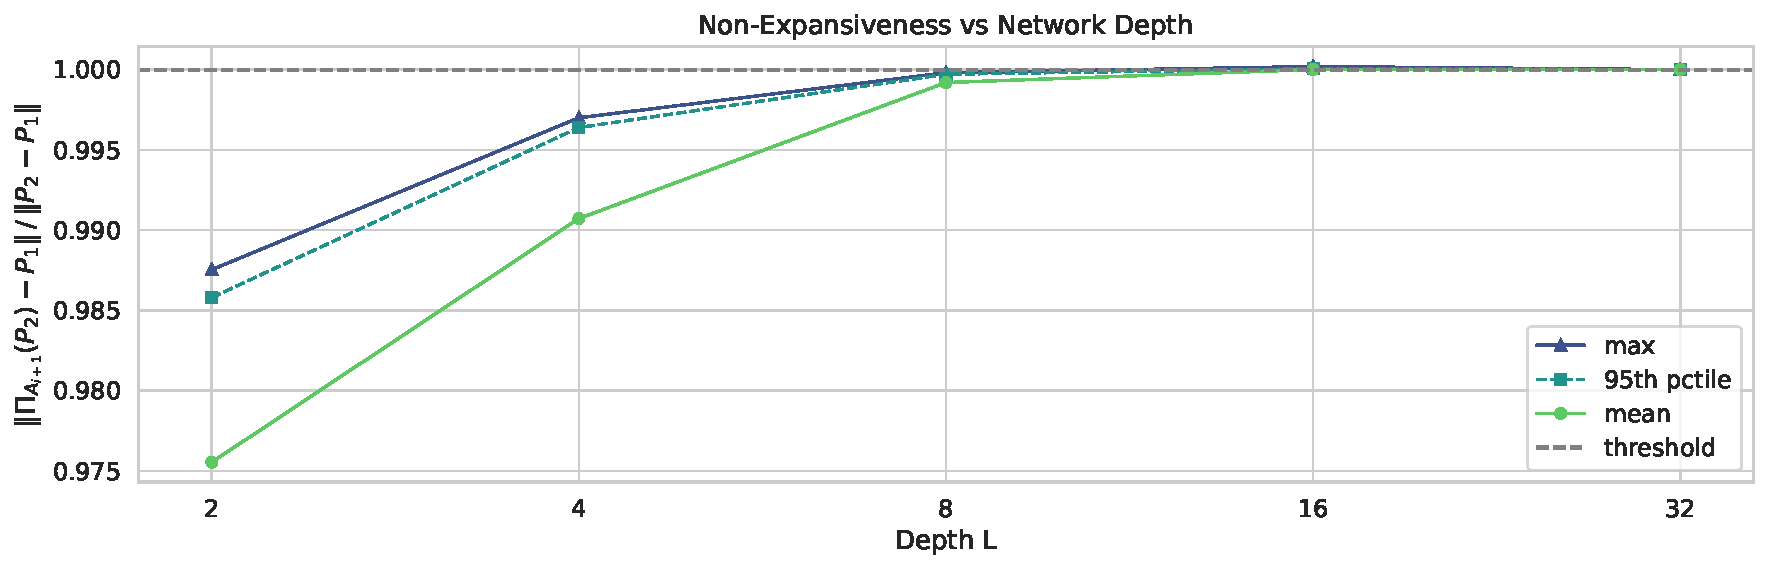
\includegraphics[width=\linewidth]{images/deep/local_nonexpansiveness_deep.pdf}
      \caption{Progression of the non-expansiveness ratio $r^{(i)}$ across varying network depths $L$. }
      \label{fig:non_expans}
  \end{figure}
The observed ratio can be seen in \cref{fig:non_expans}. This shows that the equality holds across all depths: $r^{(i)} \leq 1$ up to the solver precision, excluding the single $L = 16$ outlier at $1.0002$ whose $\delta^{(i+1)}$ sits just above the cut-off (\cref{tab:nonexp-deep}). 
\begin{table}[h]
\centering
\caption{Non-expansiveness ratio $r^{(i)}$ pooled across layers, seeds, and
  recorded steps, for depths $L \in \{2,4,8,16,32\}$ (three seeds).}
  \begin{tabular}{@{} r r r r r r @{}}
  \toprule
  $L$ & $n_{\mathrm{valid}}$ & $n_{\mathrm{vanish}}$ & $\max r$ & $\bar r$
      & $\%\{r > 1 + 10^{-5}\}$ \\
  \midrule
  $2$  & $18$ & $0$  & $0.9875$ & $0.9755$ & $0\%$    \\
  $4$  & $21$ & $13$ & $0.9970$ & $0.9907$ & $0\%$    \\
  $8$  & $18$ & $18$ & $0.9998$ & $0.9992$ & $0\%$    \\
  $16$ & $18$ & $13$ & $1.0002$ & $1.0000$ & $16.7\%$ \\
  $32$ & $9$  & $13$ & $1.0000$ & $1.0000$ & $0\%$    \\
  \bottomrule
  \end{tabular}

  \label{tab:nonexp-deep}
  \end{table}
